% !Mode:: "TeX:UTF-8"

\documentclass[UTF8,openany,twoside,fontset=fandol]{ctexbook}	% 此处使用了开源的fandol字体
% !Mode:: "TeX:UTF-8"

\usepackage[%
	a4paper,
	top=21mm,
	bottom=20.5mm,
	left=26mm,
	right=26mm,
    headsep=8.5mm,
	includehead,
	includefoot
]{geometry}					% 控制页面尺寸

\usepackage[russian,french,ngerman,main=english]{babel}	% 对俄语,法语,德语,和英语的支持
\addto\captionsenglish{     % 只有在启用babel宏包以后才能用这些命令
  \renewcommand{\figurename}{图}%
  \renewcommand{\tablename}{表}%
  \renewcommand{\bibname}{参考文献}%
}

\usepackage{xcolor}         % 支持彩色
\usepackage{iftex}          % 判定是否是某种tex引擎

\ifptexng
    \usepackage{newtxtext}  % 使用开源的模仿Times New Roman的字体
    \usepackage{bmpsize}    % ptex-ng专用的宏集
\fi

\ifxetex
% \setmainfont{Times New Roman}
\setmainfont{FreeSerif}		% 有西里尔字母
\setsansfont{FreeSans}
\setmonofont{FreeMono}

\usepackage{fontawesome5}   % 插入一些有趣的矢量图标
\usepackage{academicons}    %插入一些学术界适用的矢量图标
    \definecolor{orcidlogocol}{HTML}{A6CE39}    % ORCID的颜色
\usepackage{microtype}      % 对西文排版的改进
\fi

\usepackage[super]{nth}     % 上标形式的1st, 2nd
\usepackage{hologo}         % 插入LaTeX有关的logo
\usepackage{titletoc}       % 控制目录的宏包
\usepackage{titlesec}       % 控制标题的宏包
\usepackage{fancyhdr}       % 页眉和页脚的相关定义
\usepackage[final]{graphicx}% 处理图片
\usepackage{float}		    % 浮动体处理
\usepackage{xurl}	        % 插入改良的URL
\usepackage{verbatim}       % 将一段代码原样转义输出
\usepackage{enumitem}       % 使用enumitem宏包,改变列表项的格式
\usepackage{amsmath}        % 公式宏包
\usepackage{amssymb}		% 符号宏包
\usepackage{mathtools}      % 对AMS数学宏包的改进
\usepackage{bm}				% 处理数学公式中的黑斜体的宏包
\usepackage{esvect}         % 提供各种向量的箭头符号
\usepackage[font=footnotesize]{caption}     % 使用caption宏包设置浮动体标题
    \DeclareCaptionLabelSeparator{mysep}{\,\,\,}
    \captionsetup{labelsep=mysep}
\usepackage[caption=false,font=footnotesize]{subfig}    % 比较好的并列的浮动体宏包
\usepackage{capt-of}        % 在不是浮动体的环境内插入标题
\usepackage{pdfpages}       % 插入整页的PDF文件
\usepackage{multicol}       % 插入多个分栏的局部页面
\usepackage{siunitx}        % 正确排版数字与单位,使数字和单位的字体与上下文保持一致
    \sisetup{per-mode = symbol}
\usepackage{tabularx}		% 可伸缩表格
\usepackage{multirow}       % 表格可以合并多个row
\usepackage{diagbox}        % 在表格里打印斜线
\usepackage{booktabs}       % 表格横的粗线;\specialrule{1pt}{0pt}{0pt}
\usepackage{longtable}      % 支持跨页的表格
\usepackage{xltabular}      % 跨页表格longtable+自适应表格tabularx
\usepackage{threeparttable} % 正确插入表格内的footnote
\usepackage{zhlipsum}       % 中文乱文
\usepackage{lipsum}         % 西文乱文
\usepackage{nomencl}        % 输出缩写表
    \renewcommand{\nomname}{主要符号表} % 更改Nomenclature的名称
    \makenomenclature
    \setlength{\nomitemsep}{-\parsep}
\usepackage[chapter]{minted}% 引用代码,比较漂亮
\usepackage[referable]{threeparttablex}             % 跨页表格longtable的threeparttable
\usepackage[framemethod=tikz]{mdframed}             % 插入带框的文本
\usepackage[amsmath,thmmarks,hyperref]{ntheorem}	% 定理类环境宏包
\usepackage[sort&compress]{gbt7714}
\usepackage{csquotes}       % 各种西文的引号

% 带圆圈的脚注
\usepackage{pifont}
\usepackage[flushmargin,para,symbol*]{footmisc}
\DefineFNsymbols{circled}{{\ding{192}}{\ding{193}}{\ding{194}}
	{\ding{195}}{\ding{196}}{\ding{197}}{\ding{198}}{\ding{199}}{\ding{200}}{\ding{201}}}
\setfnsymbol{circled}

% 生成有书签的 pdf 及其开关, 该宏包应放在所有宏包的最后, 宏包之间有冲突
\usepackage[%
    bookmarksnumbered=true,
    bookmarksopen=true,
    breaklinks=true,
    pdfstartview=FitH,
    hidelinks
]{hyperref}

% 算法的宏包,注意宏包兼容性,先后顺序为float、hyperref、algorithm(2e),否则无法生成算法列表
\usepackage[plainruled,linesnumbered,algochapter]{algorithm2e}

% \pdfminorversion = 7
											% 读取package.tex文件
\graphicspath{{figures/}}										% 在figures文件夹里寻找图片,建议使用PDF格式的矢量图

%===================================== Cover and TOC =====================================
\begin{document}												% 文档开头
% !Mode:: "TeX:UTF-8"

%========================================= Font ==========================================
% 定义字号
\newcommand{\sanhao}{\fontsize{16pt}{16pt}\selectfont}      % 三号, 1.0倍行距
\newcommand{\xiaosan}{\fontsize{15pt}{15pt}\selectfont}     % 小三, 1.0倍行距
\newcommand{\sihao}{\fontsize{14pt}{14pt}\selectfont}       % 四号, 1.0倍行距
\newcommand{\xiaosi}{\fontsize{12pt}{12pt}\selectfont}      % 小四, 1.0倍行距
\newcommand{\wuhao}{\fontsize{10.5pt}{10.5pt}\selectfont}   % 五号, 1.0倍行距
\newcommand{\xiaowu}{\fontsize{9pt}{9pt}\selectfont}        % 小五, 1.0倍行距

% 默认字体
\makeatletter
\renewcommand\normalsize{
	\@setfontsize\normalsize{12pt}{12pt}
	\setlength\abovedisplayskip{8pt}
	\setlength\abovedisplayshortskip{8pt}
	\setlength\belowdisplayskip{\abovedisplayskip}
	\setlength\belowdisplayshortskip{\abovedisplayshortskip}
	\let\@listi\@listI
}

% 脚注字体为 5号
\renewcommand{\footnotesize}{\wuhao}

% 设置行距和段落间垂直距离
\setlength{\parindent}{2em}
\setlength{\parskip}{3pt plus1pt minus1pt}
\def\defaultfont{\renewcommand{\baselinestretch}{1.5}\normalsize\selectfont}

% 设置字间距,使每行37个字,若要减少每行字数(一般以34个),将0.56pt的值增加
\renewcommand{\CJKglue}{\hskip 0.56pt plus 0.08\baselineskip}

% 公式跨页设置,公式之前可以换页,公式出现在页面顶部
\predisplaypenalty=0
\allowdisplaybreaks[4]

% 允许断页时给上一页底部留有一定空白,避免拉大标题和行距
\raggedbottom

%========================================= TOC ===========================================
% 中文目录格式定义
\renewcommand\contentsname{目~~~~录}
\titlecontents{chapter}[3.8em]{\hspace{-3.8em}}{\thecontentslabel~~}{}{\titlerule*[3pt]{.}\contentspage}
\dottedcontents{section}[38pt]{}{22pt}{0.3pc}
\dottedcontents{subsection}[60pt]{}{32pt}{0.3pc}

% 英文目录格式定义: 细点\@dottedtocline  粗点\@dottedtoclinebold
\renewcommand*\l@chapter{\@dottedtocline{0}{0em}{5em}}
\renewcommand*\l@section{\@dottedtocline{1}{1em}{1.8em}}
\renewcommand*\l@subsection{\@dottedtocline{2}{2.0em}{2.5em}}
\def\@dotsep{0.75}           % 定义英文目录的点间距
\setlength\leftmargini {50pt}
\setlength\leftmarginii {50pt}
\def\engcontentsname{CONTENTS}
\newcommand\tableofengcontents{
	\@restonecolfalse
	\chapter*{\engcontentsname  %chapter*上移一行,避免在toc中出现。
		\@mkboth{%
			\engcontentsname}{\engcontentsname}}
	\@starttoc{toe}%
	\if@restonecol\twocolumn\fi
}

%======================================= Chapter =========================================
% 章节格式定义
\renewcommand\chaptername{\thechapter}
\ctexset{chapter={name={,},number={\arabic{chapter}}}}
\setcounter{secnumdepth}{4} \setcounter{tocdepth}{2}
\titleformat{\chapter}{\center\sanhao}{\chaptertitlename}{0.8em}{}
\titlespacing{\chapter}{0pt}{-5.3mm}{4.2mm}
\titleformat{\section}{\xiaosan}{\thesection}{0.5em}{}
\titlespacing{\section}{0pt}{3mm}{3mm}
\titleformat{\subsection}{\sihao}{\thesubsection}{0.5em}{}
\titlespacing{\subsection}{2.13em}{3mm}{3mm}

% 重新定义BiChapter命令,可实现标题手动换行,但不影响目录
\def\BiChapter{\relax\@ifnextchar [{\@BiChapter}{\@@BiChapter}}
\def\@BiChapter[#1]#2#3{\chapter[#1]{#2}
    \addcontentsline{toe}{chapter}{\xiaosi \thechapter\hspace{0.5em} #3}}
\def\@@BiChapter#1#2{\chapter{#1}
    \addcontentsline{toe}{chapter}{\xiaosi \thechapter\hspace{0.5em}{\boldmath #2}}}

% 定义双标题
\newcommand{\BiSection}[2]{
	\section{#1}
	\addcontentsline{toe}{section}{\protect\numberline{\csname thesection\endcsname}#2}
}
\newcommand{\BiSubsection}[2]{
	\subsection{#1}
	\addcontentsline{toe}{subsection}{\protect\numberline{\csname thesubsection\endcsname}#2}
}
\newcommand{\BiSubsubsection}[2]{
    \subsubsection{#1}
    \addcontentsline{toe}{subsubsection}{\protect\numberline{\csname thesubsubsection\endcsname}#2}
}

% 该附录命令适用于有章节的完整附录和用于发表文章和简历的附录
\newcommand{\BiAppChapter}[2]{
	\phantomsection
	\chapter{#1}
	\addcontentsline{toe}{chapter}{\xiaosi Appendix \thechapter~~#2}
}
\newcommand{\BiAppendixChapter}[2]{
	\phantomsection
	\markboth{#1}{#1}
	\addcontentsline{toc}{chapter}{\xiaosi #1}
	\addcontentsline{toe}{chapter}{\xiaosi #2}  \chapter*{#1}
}

% 参考文献格式
\bibliographystyle{gbt7714-numerical}
\addtolength{\bibsep}{-0.8em}

%======================================== Header =========================================
% 定义页眉和页脚
\newcommand{\makeheadrule}{
\rule[6pt]{\textwidth}{0.5pt} \\[-17.5pt]
\rule{\textwidth}{0.5pt}}
\renewcommand{\headrule}{
    {\if@fancyplain\let\headrulewidth\plainheadrulewidth\fi
     \makeheadrule}}
\pagestyle{fancyplain}

% 不要注销这一行,否则页眉会变成:“第1章1  绪论”样式
\renewcommand{\chaptermark}[1]{\markboth{\chaptertitlename~~\ #1}{}}
\fancyhf{}
\fancyhead[CO]{\wuhao \leftmark}
\fancyhead[CE]{\wuhao 西安交通大学博士学位论文}
\fancyfoot[LE,RO]{\xiaowu \thepage}

%======================================= Theorem =========================================
% 定理正文和标题字体
\theoremstyle{plain}
\theoremheaderfont{\heiti\rmfamily}
\theorembodyfont{\rmfamily}
\theoremseparator{:}

% 定理环境和上下文之间的距离
\setlength{\theorempreskipamount}{8pt}
\setlength{\theorempostskipamount}{8pt}

% 定义新的定理环境
\theoremsymbol{$\Diamond$} \newtheorem{definition}{\hskip 2em \heiti 定义}[chapter]
\theoremsymbol{$\blacklozenge$} \newtheorem{example}{\hskip 2em \heiti 例}[chapter]
\theoremsymbol{$\square$} \newtheorem{theorem}{\hskip 2em \heiti 定理}[chapter]
\theoremsymbol{$\blacksquare$} \newtheorem*{proof}{\hskip 2em \heiti 证明}

%========================================= FTE ===========================================
% 图表公式的编号为1-1格式,子图编号为 (a) 的格式
\renewcommand{\thefigure}{\arabic{chapter}-\arabic{figure}}
\renewcommand{\thetable}{\arabic{chapter}-\arabic{table}}
\renewcommand{\theequation}{\arabic{chapter}-\arabic{equation}}

% 把 tabularx 宏包的列格式左对齐改成居中对齐
\newcolumntype{Y}{>{\centering\arraybackslash}X}

% 调整罗列环境的布局
\setitemize{leftmargin=3em,itemsep=0em,partopsep=0em,parsep=0em,topsep=-0em}
\setenumerate{leftmargin=3.2em,itemsep=0em,partopsep=0em,parsep=0em,topsep=0em}

% 更改算法标题
\SetAlCapSty{textrm}
\SetAlCapFnt{\wuhao}
\SetAlCapNameFnt{\wuhao}
\SetAlgoCaptionSeparator{\,\,}
\SetAlCapSkip{10pt}
\renewcommand\thealgocf{\csname the\algocf@within\endcsname-\@arabic\c@algocf}
\makeatother

% 更改代码标题
\renewcommand{\listingscaption}{代码}
\renewcommand*{\thelisting}{\thechapter-\arabic{listing}}
% \renewcommand{\lstlistingname}{代码}
% \renewcommand{\thelstlisting}{\arabic{chapter}-\arabic{lstlisting}} 											% 读取format.tex文件

\frontmatter
% !Mode:: "TeX:UTF-8"

\begin{titlepage}
	% 中文封面
	\begin{center}
		\begin{figure*}[!ht]\vspace{4.5em}
			\centering
			\includegraphics[width=0.5\textwidth]{xjtu}
		\end{figure*}
		
		\vspace{1.5em}
		\begin{center} {\zihao{2} 博士学位论文} \end{center}
		
		\vspace{8.5em}
		\begin{center} {\sanhao\bfseries{西安交通大学博士学位论文\hologo{LaTeX}模板}}\end{center}
		
		\vspace{16em}
		{\sanhao
			\begin{center} \renewcommand{\arraystretch}{1.8}
				\begin{tabular}{c}
					学位申请人:XXX \\
					指导教师:XXX\,\,\,教授 \\
					合作导师:XXX\,\,\,教授 \\
					学科名称:XXX \\
					XXXX年XX月 \\
				\end{tabular} \renewcommand{\arraystretch}{1}
			\end{center}
		}
	\end{center}
	\clearpage{\pagestyle{empty}\cleardoublepage}
	
	%---------------------------------------------------------------------------------
	% 英文封面
	\newpage\thispagestyle{empty}
	\begin{center}
		\parbox[t][0.4cm][t]{\textwidth}{}
		
		\begin{center}{\sanhao\bfseries \hologo{LaTeX} Template for Doctoral Dissertation of XJTU}\end{center}
		
		\vspace{4.1cm}
		{\sanhao
			\begin{center} \renewcommand{\arraystretch}{1.35}
				\begin{tabular}{c}
					A dissertation submitted to  \\
					Xi'an Jiaotong University \\
					in partial fulfillment of the requirements \\
					for the degree of \\
					Doctor of Philosophy \\
				\end{tabular} \renewcommand{\arraystretch}{1}
			\end{center}
		}
		
		\vspace{1.4cm}
		{\sanhao
			\begin{center} \renewcommand{\arraystretch}{1.35}
				\begin{tabular}{c}
					By \\
					XXX (名在前,姓在后,例如 Ming Zhang) \\
					Supervisor: Prof.\ XXX (导师姓名全拼,例如 Anxue Zhang) \\
					Associate Supervisor: Prof.\ XXX (导师姓名全拼,例如 Anxue Zhang) \\
					XXXXXX (学科名称,例如:Electronic Science and Technology) \\
					XXX XXXX (英文日期,月在前,年在后,例如:September 2017) \\
				\end{tabular} \renewcommand{\arraystretch}{1}
			\end{center}
		}
	\end{center}
	\clearpage{\pagestyle{empty}\cleardoublepage}
	
	%---------------------------------------------------------------------------------
	% 答辩委员会
	\newpage\thispagestyle{empty}

\newgeometry{
	a4paper,
	top=21mm,
	bottom=19mm,
	left=26mm,
	right=26mm,
    headsep=5.5mm,
	includehead,
	includefoot
}

	\begin{center}
		\parbox[t][0cm][t]{\textwidth}{}
		
		\begin{center}{\zihao{3}\bfseries{博士学位论文答辩委员会}}\end{center}
		
		\vspace{1cm}
		\begin{center}{\zihao{3}\bfseries{西安交通大学博士学位论文\hologo{LaTeX}模板}}\end{center}
		
		\vspace{5.4cm}
		{\sanhao
			\begin{center} \renewcommand{\arraystretch}{1.5}
				\begin{tabular}{l}
					答辩人: XXX \\
					答辩委员会委员:\\
					\hspace{2em} XXXX大学\,XXX教授: \underline{\hspace{6em}}(主席)\\
					\hspace{2em} XXXX大学\,XXX教授: \underline{\hspace{6em}} \\
					\hspace{2em} XXXX大学\,X\quad X教授: \underline{\hspace{6em}} \\
					\hspace{2em} XXXX大学\,XXX教授: \underline{\hspace{6em}} \\
					\hspace{2em} XXXX大学\,XXX教授: \underline{\hspace{6em}} \\
					答辩时间: XXXX年XX月XX日 \\
					答辩地点: 西安交通大学兴庆校区XXX \\
				\end{tabular} \renewcommand{\arraystretch}{1}
			\end{center}
		}
	\end{center}
	
	\restoregeometry
	\clearpage{\pagestyle{empty}\cleardoublepage}
\end{titlepage}
												% 封面
% !Mode:: "TeX:UTF-8"

%====================================== 中文摘要 ==========================================
\BiAppendixChapter{摘~~~~要}{ABSTRACT (Chinese)}
\setcounter{page}{1}\pagenumbering{Roman}
\defaultfont

博士学位论文摘要正文为 1000 字左右。

内容一般包括:从事这项研究工作的目的和意义;完成的工作(作者独立进行的研究工作及相应结果的概括性叙述);获得的主要结论(这是摘要的中心内容)。博士学位论文摘要应突出论文的创新点。

摘要中一般不用图、表、化学结构式、非公知公用的符号和术语。

如果论文的主体工作得到了有关基金资助,应在摘要第一页的页脚处标注:本研究得到某某基金(编号:)资助。


\vspace{\baselineskip}
\noindent{\fontsize{11.5pt}{11.5pt}\selectfont\bfseries 关\hspace{0.5em}键\hspace{0.5em}词}:西安交通大学,博士学位论文,\hologo{LaTeX}模板

\vspace{\baselineskip}
\noindent{\fontsize{11.5pt}{11.5pt}\selectfont\bfseries 论文类型}:应用基础

\clearpage

%====================================== 英文摘要 ==========================================
\BiAppendixChapter{ABSTRACT}{ABSTRACT (English)}

\noindent 英文摘要正文每段开头不缩进,每段之间空一行。\newline

\noindent The abstract goes here. \newline

\noindent \hologo{LaTeX} is a typesetting system that is very suitable for producing scientific and mathematical documents of high typographical quality.

\vspace{\baselineskip}
\noindent{\fontsize{11.5pt}{11.5pt}\selectfont\bfseries KEY WORDS}: Xi'an Jiaotong University, Doctoral dissertation, \hologo{LaTeX} template

\vspace{\baselineskip}
\noindent{\fontsize{11.5pt}{11.5pt}\selectfont\bfseries TYPE OF DISSERTATION}: Application Fundamentals

\clearpage


\newpage 
%\clearpage{\pagestyle{empty}\cleardoublepage}% 正文章节从奇数页开始											% 摘要
% !Mode:: "TeX:UTF-8" 

%====================================== 中文目录 ==========================================
\defaultfont
\pdfbookmark[0]{目~~~~录}{mulu}
\tableofcontents
\noindent 声\quad 明
\clearpage

%====================================== 英文目录 ==========================================
\pdfbookmark[0]{Contents}{econtent}
\tableofengcontents
\noindent Declarations
\clearpage{\pagestyle{empty}\cleardoublepage}% 正文章节从奇数页开始
											% 中英文目录
\nomenclature[01]{$C_v$}{灌水器流量偏差系数}
\nomenclature[02]{$D$}{管道内径 / \si{\milli\meter}}
\nomenclature[03]{$D_e$}{灌水器流道当量直径 / \si{\milli\meter}}
\nomenclature[04]{$l$}{管长 / \si{\meter}}
\nomenclature[05]{$n$}{迷宫流道单元个数 / 个}
\nomenclature[06]{$q$}{灌水器流量 / \si{\liter\per\hour}}
\nomenclature[07]{$q_n$}{灌水器额定流量 / \si{\liter\per\hour}}
\nomenclature[08]{$R_e$}{雷诺数}
\nomenclature[09]{$S_q$}{灌水器流量标准偏差}
\nomenclature[10]{$\nu$}{流体的运动粘性系数}
\nomenclature[11]{$x$}{流态指数}
\nomenclature[12]{GB/T 3102.11-1993}{\href{http://openstd.samr.gov.cn/bzgk/gb/newGbInfo?hcno=3DE79450D562E62D41CB6E79FF411054}{物理科学和技术中使用的数学符号}(见附件)}
\nomenclature[13]{GB/T 7714-2015}{\href{http://openstd.samr.gov.cn/bzgk/gb/newGbInfo?hcno=7FA63E9BBA56E60471AEDAEBDE44B14C}{信息与文献 参考文献著录规则}}
										% 符号缩写表
\printnomenclature[5cm]											% 排版nomenclature
\addcontentsline{toe}{chapter}{Abbreviations and Symbols}		% 西文的符号缩写表命名,中文的名称请在package.tex里更改

%======================================= Main Body =======================================
\mainmatter
%!Mode::"TeX:UTF-8"

\BiChapter{\hologo{LaTeX}介绍}{Introduction of \hologo{LaTeX}}

本章对\hologo{LaTeX}排版系统做一个简要介绍,希望没有使用过\hologo{LaTeX}的同学对\hologo{LaTeX}有一个初步认识。

%=========================================================================================
\BiSection{\hologo{LaTeX}是什么?}{What is \hologo{LaTeX}?}

\hologo{LaTeX}是一款排版系统,和其它排版软件例如Word相比,\hologo{LaTeX}具有非常明显的优势和不足。其最大的优势是高质量、高水准的专业排版效果;最大的缺点是使用门槛高,需要具备一定的编程基础\footnote{因为\hologo{LaTeX}的资源非常丰富,有许多模板可以使用,这些模板已经为用户定制好了排版格式,所以单纯从使用的角度看,使用\hologo{LaTeX}的门槛其实并不算高。}。对于习惯于抽象思维的科技人员而言,与精美的排版效果相比,\hologo{LaTeX}的确缺点是微不足道的,只要经过短时间(一周足已)的学习和实践,就可以编写出高质量的科研论文。

\hologo{LaTeX}的基础是\hologo{TeX},\hologo{TeX}诞生于20世纪70年代末到80年代初,用来排版高质量的书籍,特别是包含数学公式的书籍。有趣的是,这样一款排版软件并非在排版业界产生,而是由著名计算机科学家Donald Ervin Knuth(中文名高德纳)在修订其七卷巨著《计算机程序设计艺术》时设计的。

虽然\hologo{TeX}功能非常强大,但是多达900多条的排版命令让排版人员使用起来非常不便。因此20世纪80年代初,Leslie Lamport博士给\hologo{TeX}编写了一组自定义命令宏包,并取名为\hologo{LaTeX},其中La是其姓名的前两个字母。\hologo{LaTeX}拥有比原来的\hologo{TeX}更为规范的格式命令和一整套预定义的格式,可以让完全不懂排版技术的学者们很容易地将书籍和文稿排版出来。\hologo{LaTeX}一出,很快风靡全球,在1994年\hologo{LaTeXe}完善之后,现在已经成为国际上数学、物理、计算机等科技领域专业排版的事实标准,相关专业的学术期刊也都采用\hologo{LaTeX}作为投稿格式。

%-----------------------------------------------------------------------------------------
\BiSection{为什么用\hologo{LaTeX}?}{Why use \hologo{LaTeX}?}

虽然论文排版是一项基本技能,但是从实际情况看,同学们经常被各种格式整得晕头转向。加之Word排版不够美观,版本管理麻烦,排版效率低下,因此开发\hologo{LaTeX}论文模板非常重要。国际上许多著名的出版机构和学术期刊都有自己的\hologo{LaTeX}模板,国内外许多高效也有自己的硕博论文\hologo{LaTeX}模板。事实上,\hologo{LaTeX}已经成为科技出版行业的国际标准,特别是数学、物理、计算机和电子信息学科。

采用\hologo{LaTeX}排版主要有以下优点:
\begin{enumerate}	
    \item 排版质量高:主要体现在对版面尺寸的严格控制,对字距、行距和段距等间距的松紧适度掌握,对数学公式的精细设计,对插图和表格的灵活处理,对代码和算法的优美呈现,等等。
    \item 安全稳定:自发布以来\hologo{TeX}和\hologo{LaTeX}没有发现系统漏洞,不会出现死机或者系统崩溃而导致编写的内容来不及保存。
    \item 灵活方便:\hologo{LaTeX}的源文件是纯文本文件,文件大小比Word小很多,不会因为文容的增加而导致文档打开、编辑、保存和关闭等操作变慢。因为\hologo{LaTeX}在编译时才将所有源文件和图表汇总,故撰写内容时可以随意增删章节和图表。并且和大部分程序设计语言一样,\hologo{LaTeX}具有注释功能,作者可以在源文件任何地方添加注释,而不会影响最终生成的文档。
    \item 格式和内容分离:\hologo{LaTeX}将文档格式和文档内容分开处理,作者只要选择合适的模板,就可专心致志地撰写文档内容,文档的格式细节则由\hologo{LaTeX}模板统一规划设置。特别是文献管理能力非常强大,这给撰写像博士论文一样需要大量引用参考文献的文档提供了很大便利。
	\item 免费开源:\hologo{LaTeX}软件完全免费,源代码也全部公开,并且相应的配套软件也都采用开源的方式。
\end{enumerate}

无论你是因为羡慕\hologo{LaTeX}漂亮的输出结果,还是因为要给学术期刊投稿而被逼上梁山,都不得不面对这样一个事实:\hologo{LaTeX}是一种并不简单的排版软件,不可能只点点鼠标就弄好一篇漂亮的文章。还得拿出点搞研究的精神,通过不断练习,才能编排出整齐漂亮的论文。一旦你掌握了如何使用\hologo{LaTeX}撰写出精美漂亮的论文时,你会发现你的决定是明智的,你的投入是值得的。

%=========================================================================================
\BiSection{怎样用\hologo{LaTeX}?}{How to use \hologo{LaTeX}?}

本模板在Windows + \hologo{TeX}Live 2020\footnote{每年发布新版本} + \Hologo{TeX}Studio平台下开发,采用\hologo{XeLaTeX}引擎或者p\hologo{TeX}-ng引擎编译。虽然之前也开发过一个基于C\hologo{TeX}的模板,但是经过多方面比较发现\hologo{TeX}Live+\hologo{XeLaTeX}处理中文更好,所以基于C\hologo{TeX}的模板没有共享。

{\color{red}本模板不能在C\hologo{TeX}软件下使用,必须采用\hologo{TeX}Live,并且编译方式是\hologo{XeLaTeX}。\hologo{TeX}Live每年更新一个版本,我用的是\hologo{TeX}Live 2020。文本编辑器可以根据自己的喜好选用,我用的是\hologo{TeX}Studio,这款开源软件非常不错,推荐大家使用。还有其他\url{https://tex.stackexchange.com/questions/339/latex-editors-ides}}

本模板的源文件通过主目录下的\texttt{main.tex}统一管理,\texttt{setup}文件夹中存放格式定义和封面、摘要、目录等内容,\texttt{body}文件夹中存放论文正文章节的源文件,appendix文件夹中存放附录、致谢和声明等内容。

\begin{mdframed}
本模板只提供论文的格式定义,不提供\hologo{LaTeX}的详细使用方法。
因为\hologo{LaTeX}的资源非常丰富,大家可以在网上查找资料和并参与讨论,这样学习效率更高。我参考的两本书是《\hologo{LaTeX}入门》\cite{Liu_2013_LaTeXRuMen}和《一份(不太)简短的\hologo{LaTeX2e}介绍》\cite{Oetiker_2019_YiFenBuTaiJianDuanDeLaTeX2eJieShao},还有《\hologo{LaTeX}科技文档排版》\cite{Gai_2005_LaTeXKeJiWenDangPaiBan}和《\hologo{LaTeX2e}插图指南》\cite{Reckdahl_2017_LaTeX2eChaTuZhiNan}。
\end{mdframed}

%!Mode::"TeX:UTF-8"

\BiChapter{图表公式排版}{Figures, Tables, and Equations}

虽然本模板不讲解\hologo{LaTeX}的详细使用方法,但是为了方便大家使用本模板撰写论文,本章对论文写作中经常用到的{\heiti 图、表、公式}等内容的排版方法做一个简单介绍。

\begin{mdframed}
本模板基于\texttt{ctex}宏包,强烈建议仔细阅读。

交大的论文指南和模板都没有涉及到算法和代码的排版,所以本模板自行设计了一些样式。

建议在\texttt{Overleaf}网站上测试,最后在本地电脑上排版,使用\texttt{Times New Roman}和\texttt{fontset = windows}。

本模板对原作者Zhang Ming博士提交给研究生院的模板做了改良。
\begin{enumerate}
  \item 默认启用\texttt{newtxtext}宏包以使用其类似\texttt{Times New Roman}的开源字体;
  \item 默认启用了\texttt{microtype}宏包以改善西文排版;
  \item 默认启用了babel宏包,有兴趣的人也可以使用FreeSerif和fandol开源字体,排版包括俄语在内的多种语言;
  \item 默认启用了\texttt{hologo}宏包以输出各种\hologo{TeX}有关的符号;
  \item 默认启用了\texttt{xurl}宏包以改善URL排版;
  \item 默认启用了\texttt{mathtools}宏包以改善最为广泛使用的\texttt{amsmath}宏包一些不足;
  \item 默认启用了\texttt{bm}和\texttt{esvect}宏包以改善某些数学公式的排版;
  \item 默认启用了\texttt{ulem}和\texttt{csquotes}宏包以改善某些文本的排版;
  \item 默认启用了\texttt{caption}宏包和\texttt{subfig}宏包以提供最佳的多浮动体和题注的排版;
  \item 默认启用了\texttt{capt-of}宏包在不是浮动体的环境内插入题注;
  \item 默认启用了\texttt{academicons}和\texttt{fontawesome5}宏包以插入一些矢量图标;
  \item 默认启用了\texttt{multicol}宏包以提供局部的多栏环境;
  \item 默认启用了\texttt{siunitx}宏包以正确排版数字和单位;
  \item 默认启用了\texttt{longtable}, \texttt{xltabular}, \texttt{threeparttable}, 和\texttt{threeparttablex}宏包以提供跨页的、带有注释的复杂表格;
  \item 默认启用了\texttt{zhlipsum}和\texttt{lipsum}宏包以提供中西文乱文;
  \item 默认启用了\texttt{nomencl}宏包以排版符号缩写表;
  \item 默认启用了\texttt{mdframed}宏包以排版带框的文本;
  \item 默认启用了\texttt{minted}宏包以提供更简单美观的代码环境,编译时要注意 
  
  \verb|xelatex --shell-escape main.tex|;
  
  \item 默认更新了\hologo{BibTeX}的样式 \verb|gbt7714-numerical.bst|,要注意的是国家标准将文献中的西文作者名字都大写,而交大的模板却是将西文作者名字小写。如果需要修改,把 \verb|gbt7714-numerical.bst| 的 \verb|#1 'uppercase.name :=| 改成 \verb|#0 'uppercase.name :=| 即可。
\end{enumerate}

请读者使用本模板前仔细阅读交大的论文规范。
\end{mdframed}

%=========================================================================================
\BiSection{图}{Figures}
\BiSubsection{单幅图}{Single Figure}

图~\ref{fig_ch2_echoes} 是用\hologo{TeX}Live自带的宏包Ti\textit{k}z绘制而成,Visio画不出这么好看的图。
\begin{figure}[!ht]
	\centering
	\includegraphics[width=\linewidth]{echoes}
	\caption{雷达回波信号({\color{red}注意}:图注是五号字)。}\label{fig_ch2_echoes}
\end{figure}

%-----------------------------------------------------------------------------------------
\BiSubsection{多幅图}{Multiple Figures}

如果一幅图中包含多幅子图,每一幅子图都要有图注,并且子图用(a)、(b)、(c)等方式编号,如图~\ref{fig_ch2_badge} 所示。
\begin{figure}[!ht]
	\centering
	\subfloat[灰色的交大校徽]{\includegraphics[width=0.45\textwidth]{xjtu_gray}}
	\hfill
	\subfloat[蓝色的交大校徽]{\includegraphics[width=0.45\textwidth]{xjtu_blue}}
	\caption{交大校徽\label{fig_ch2_badge}}
\end{figure}

%=========================================================================================
\BiSection{表}{Tables}

表格要求采用三线表,与文字齐宽,顶线与底线线粗是$1\frac{1}{2}$磅,中线线粗是1磅,如表~\ref{tab_ch2} 所示\footnote{{\color{red}注意}:图表中的变量与单位通过斜线 / 隔开。}。
\begin{table}[!htb]
	% \renewcommand{\arraystretch}{1.2}
	\centering\wuhao
	\caption{表题也是五号字}\label{tab_ch2} %\vspace{2mm}
	\begin{tabularx}{\linewidth}{@{}YYYY@{}}
	\toprule[1.5pt]
		Interference & DOA/degree & Bandwidth/MHz & INR/dB\\
	\midrule[1pt]
		1 & -30 & 20 & 60\\
		2 & 20 & 10 & 50\\
		3 & 40 & 5 & 40\\
	\bottomrule[1.5pt]
	\end{tabularx}
\end{table}

%=========================================================================================
\BiSection{公式}{Equations}
\BiSubsection{单个公式}{Equations}

\hologo{LaTeX}最强大的地方在于对数学公式的编辑,不仅美观,而且高效。单个公式的编号如式~(\ref{equ_ch2_pdf}) 所示,该式是正态分布的概率密度函数\cite{Manolakis2005},
\begin{equation}\label{equ_ch2_pdf}
	f_Z(z)=\frac{1}{\pi\sigma^2}\exp\left(-\frac{|z-\mu|^2}{\sigma^2}\right)
\end{equation}
式中:$\mu$是Gauss随机变量$Z$的均值;$\sigma^2$是$Z$的方差。

%-----------------------------------------------------------------------------------------
\BiSubsection{多个公式}{Subequations}

多个公式作为一个整体可以进行二级编号,如式~(\ref{equ_ch2_fourier}) 所示,该式是连续时间Fourier变换的正反变换公式\cite{Vetterli2014},
\begin{subequations}\label{equ_ch2_fourier}
	\begin{align}
		X(f)&=\int_{-\infty}^{\infty}x(t)e^{-j2\pi f t}\mathrm{d}t\\
		x(t)&=\int_{-\infty}^{\infty}X(f)e^{j2\pi f t}\mathrm{d}f
	\end{align}
\end{subequations}
式中:$x(t)$是信号的时域波形;$X(f)$是$x(t)$的Fourier变换。

如果公式中包含推导步骤,可以只对最终的公式进行编号,例如:
\begin{align}
	\bm{w}_{\mathrm{smi}}&=\alpha\left[\frac{1}{\sigma_n^2}\bm{v}(\theta_0)- \frac{1}{\sigma_n^2}\bm{v}(\theta_0)+\sum_{i=1}^{N}\frac{\bm{u}_i^H\bm{v}(\theta_0)}{\lambda_i} \bm{u}_i\right]\nonumber\\
	&=\frac{\alpha}{\sigma_n^2}\left[\bm{v}(\theta_0)- \sum_{i=1}^{N}\bm{u}_i^H\bm{v}(\theta_0)\bm{u}_i+ \sum_{i=1}^{N}\frac{\sigma_n^2\bm{u}_i^H\bm{v}(\theta_0)}{\lambda_i}\bm{u}_i\right]\nonumber\\
	&=\frac{\alpha}{\sigma_n^2}\left[\bm{v}(\theta_0)-\sum_{i=1}^{N} \frac{\lambda_i-\sigma_n^2}{\lambda_i}\bm{u}_i^H\bm{v}(\theta_0)\bm{u}_i\right]
\end{align}

%!Mode::"TeX:UTF-8"

\BiChapter{多语言排版}{Multilingual Typesetting}

\BiSection{标题2}{section}

1)标题 4

(1)标题 5

a)标题 6

b)标题 6

(a)标题 7

\BiSubsection{标题3}{subsection}

The United States of America (USA), commonly known as the United States (U.S. or US), or America, is a country primarily located in North America, consisting of 50 states, a federal district, five major self-governing territories, and various possessions. At 3.8 million square miles (9.8 million square kilometers), it is the world's third- or fourth-largest country by total area. With a population of over 328 million, it is the third most populous country in the world. The national capital is Washington, D.C., and the most populous city is New York City.

\begin{otherlanguage}{french}
La France, en forme longue depuis 1875 la République française, est un État souverain transcontinental dont le territoire métropolitain est situé en Europe de l'Ouest. Ce dernier a des frontières terrestres avec la Belgique, le Luxembourg, l'Allemagne, la Suisse, l'Italie, l'Espagne et les deux principautés d'Andorre et de Monaco. La France dispose aussi d'importantes façades maritimes sur l'Atlantique et la Méditerranée. Son territoire ultramarin s'étend dans les océans Indien, Atlantique et Pacifique ainsi qu'en Amérique du Sud, et a des frontières terrestres avec le Brésil, le Suriname et les Pays-Bas.
\end{otherlanguage}

\begin{otherlanguage}{russian}
Европейская часть России расположена на Восточно-Европейской платформе. В её основе залегают магматические и метаморфические породы докембрия. Территория между Уральскими горами и рекой Енисей занята молодой Западно-Сибирской платформой. Восточнее Енисея находится древняя Сибирская платформа, простирающаяся до реки Лены и соответствующая, в основном, Средне-Сибирскому плоскогорью. В краевых частях платформ имеются залежи нефти, природного газа, угля. К складчатым областям России принадлежат Балтийский щит, Урал, Алтай, Урало-Монгольский эпипалеозойский складчатый пояс, северо-западную часть Тихоокеанского складчатого пояса и небольшой отрезок внешней зоны Средиземноморского складчатого пояса. Самые высокие горы Кавказ приурочены к более молодым складчатым областям. В складчатых областях находятся основные запасы металлических руд.
\end{otherlanguage}

\begin{otherlanguage}{ngerman}
Deutschland (Vollform: Bundesrepublik Deutschland) ist ein Bundesstaat in Mitteleuropa. Er besteht seit 1990 aus 16 Ländern und ist als freiheitlich-demokratischer und sozialer Rechtsstaat verfasst. Die 1949 gegründete Bundesrepublik Deutschland stellt die jüngste Ausprägung des deutschen Nationalstaates dar. Deutschland hat 83 Millionen Einwohner und zählt mit durchschnittlich 233 Einwohnern pro \si{\square\kilo\meter} zu den dicht besiedelten Flächenstaaten.
\end{otherlanguage}

%!Mode::"TeX:UTF-8"

\BiAppendixChapter{致\quad 谢}{Acknowledgements}

致谢中主要感谢导师和对论文工作有直接贡献和帮助的人士和单位。致谢言语应谦虚诚恳,实事求是,字数不超过1000汉字。

\vspace{1em}
{\color{red}用于盲审的论文,此页内容全部隐去}。


%======================================= Reference =======================================
\wuhao\selectfont
\addcontentsline{toc}{chapter}{参考文献}
\addcontentsline{toe}{chapter}{References}
\bibliography{bib/mybib}

%======================================= Appendix ========================================
% !Mode:: "TeX:UTF-8"

\appendix
\defaultfont
\renewcommand{\appendixname}{附录 \Alph{chapter}}
\ctexset{chapter={name={附录}}}

\renewcommand{\thefigure}{\Alph{chapter}-\arabic{figure}}
\renewcommand{\thetable}{\Alph{chapter}-\arabic{table}}
\renewcommand{\theequation}{\Alph{chapter}-\arabic{equation}}

%!Mode::"TeX:UTF-8"

\BiAppChapter{公式定理证明}{Proofs of Equations and Theorems}

附录编号依次编为附录A,附录B。附录标题各按一级标题编排。附录中的图、表、公式另行编排序号,编号前加``附录A-''字样。这部分内容非强制性要求,如果论文中没有附录,可以省略。

排版数学定理等环境时最好给环境添加结束符,以明确定理等内容的起止标志,方便阅读。官方模板未对这些内容进行规范,本模板中定义的结束符采用$\Diamond$,例子的结束符采用$\blacklozenge$,定理的结束符采用$\square$,证明的结束符采用$\blacksquare$。

\begin{definition}[向量空间]
	设$X$是一个非空集合,$\mathbb{F}$是一个数域(实数域$\mathbb{R}$或者复数域$\mathbb{C}$)。如果在$X$上定义了加法和数乘两种运算,并且满足以下8条性质:
	%
	\begin{enumerate}
		\item 加法交换律,$\forall~x,y \in X$,$x+y = y+x \in X$;
		\item 加法结合律,$\forall~x,y,z \in X$,$(x+y)+z = x+(y+z)$;
		\item 加法的零元,$\exists~0 \in X$,使得 $\forall~x \in X$,$0+x = x$;
		\item 加法的负元,$\forall~x \in X$,$\exists~-x \in X$,使得 $x+(-x) = x-x = 0$。
		\item 数乘结合律,$\forall~\alpha,\beta \in \mathbb{F}$,$\forall~x \in X$,$(\alpha\beta)x = \alpha(\beta x) \in X$;
		\item 数乘分配律,$\forall~\alpha \in \mathbb{F}$,$\forall~x,y \in X$,$\alpha(x+y) = \alpha x + \alpha y$;
		\item 数乘分配律,$\forall~\alpha,\beta \in \mathbb{F}$,$\forall~x \in X$,$(\alpha+\beta)x = \alpha x + \beta x$;
		\item 数乘的幺元,$\exists~1 \in \mathbb{F}$,使得 $\forall~x \in X$,$1 x = x$,
	\end{enumerate}
	%
	那么称$X$是数域$\mathbb{F}$上的一个{\heiti 向量空间}(linearspace)。
\end{definition}

\begin{example}[矩阵空间]
	所有$m\times n$的矩阵在普通矩阵加法和矩阵数乘运算下构成一个向量空间$\mathbb{C}^{m\times n}$。如果定义内积如下:
	%
	\begin{equation}
	\langle A,B\rangle=\mathrm{tr}(B^HQA)=\sum_{i=1}^{n}b_i^HQa_i
	\end{equation}
	%
	其中$a_i$和$b_i$分别是$A$和$B$的第$i$列,而$Q$是Hermite正定矩阵,那么$\mathbb{C}^{m\times n}$构成一个Hilbert空间。
\end{example}

\begin{theorem}[Riesz表示定理]
	设$H$是Hilbert空间,$H^{\ast}$是$H$的对偶空间,那么对$\forall~f\in H^{\ast}$,存在唯一的$x_f\in H$,使得
	%
	\begin{equation}
	f(x)=\langle x,x_f\rangle,\qquad\forall~x\in H
	\end{equation}
	%
	并且满足$\|f\|=\|x_f\|$。
\end{theorem}

\begin{proof}
	先证存在性,再证唯一性,最后正~$\|f\|=\|x_f\|$。
\end{proof}

% !Mode:: "TeX:UTF-8"

\BiAppChapter{算法与代码}{Algorithms and Codes}

对于数学、计算机和电子信息专业,算法和代码也是经常用到的排版技巧。

%=========================================================================================
\BiSection{算法}{Algorithms}

算法描述使用algorithm2e宏包,效果如算法~\ref{alg_appB_lms} 所示。

\begin{algorithm}
\wuhao
    \SetAlgorithmName{算法}
	\IncMargin{2em}
	\DontPrintSemicolon
	\KwIn{$\bm{x}(k), \quad \mu, \quad \bm{w}(0)$}
	\KwOut{$y(k), \quad \varepsilon(k)$}
	%
	\For{$k=0,1,\cdots$}{
		$y(k) = \bm{w}^H(k)\bm{x}(k)$ \tcp*{output signal}
		$\varepsilon(k) = d(k)-y(k)$ \tcp*{error signal}
		$\bm{w}(k+1) = \bm{w}(k)+\mu\varepsilon^{\ast}(k)\bm{x}(k)$ \tcp*{weight vector update}
	}
    \caption{LMS~算法详细描述}\label{alg_appB_lms}
\end{algorithm}
%=========================================================================================
\BiSection{代码}{Codes}

源代码使用minted宏包,LMS算法的Verilog模块端口声明如代码~\ref{code_appB_lms} 所示。

\begin{listing}
\begin{minted}[linenos=true,mathescape,breaklines,breakafter=d,frame=single,fontsize=\footnotesize]{Verilog}
module stap_lms
    #(
    parameter   M                   = 4,    // number of antennas
                L                   = 5,    // length of FIR filter
                W_IN                = 18,   // wordlength of input data
                W_OUT               = 18,   // wordlength of output data
                W_COEF              = 20    // wordlength of weights
    )(
    output  signed  [W_OUT-1:0]     y_i,    // in-phase component of STAP output
    output  signed  [W_OUT-1:0]     y_q,    // quadrature component of STAP output
    output                          vout,   // data valid flag of output (high)
    input           [M*W_IN-1:0]    u_i,    // in-phase component of M antennas
    input           [M*W_IN-1:0]    u_q,    // quadrature component of M antennas
    input                           vin,    // data valid flag for input (high)
    input                           clk,    // clock signal
    input                           rst     // reset signal (high)
    );
\end{minted}
\caption{\,空时LMS算法Verilog模块端口声明}
\label{code_appB_lms}
\end{listing}



% !Mode:: "TeX:UTF-8"

\BiAppChapter{复杂表格、图片和分栏}{Complicated Tables, Figures, and Multiple Columns}

%=========================================================================================
\BiSection{复杂表格}{Complicated Tables}

请用\url{https://www.tablesgenerator.com/}生成表格

\begin{table}[H]
%   \renewcommand{\arraystretch}{1.2}
  \centering\wuhao
    \begin{threeparttable}
        \caption{一些来自fontawesome5和academicons宏包的矢量图标}\label{Alphabet}
            \begin{tabularx}{\linewidth}{@{}YYY@{}}
                \toprule[1.5pt]
                \diagbox{A1}{A2}{A3} & B\tnote{1} & C\tnote{2} \\
                \midrule[1pt]
                微信图标 \faWeixin & CV \aiCV & research gate \aiResearchGate \\
                overleaf \aiOverleaf & orcid \textcolor{orcidlogocol}{\aiOrcid} & open access \aiOpenAccess \\
                \bottomrule[1.5pt]
            \end{tabularx}
            \begin{tablenotes}
                \item[1] B1
                \item[2] C2
            \end{tablenotes}
    \end{threeparttable}
\end{table}


\begin{ThreePartTable}
\begin{TableNotes}
\item[a] \label{tn:a} test test test test test test test test
\item[b] \label{tn:b} test2
\source Made up by daleif
\end{TableNotes}
% \renewcommand{\arraystretch}{1.2}
\centering\wuhao
\begin{xltabular}{\linewidth}{@{}YYY@{}}
\caption{一个使用threeparttablex宏包制作的跨页的表格} \label{tab:long} \\

\toprule[1.5pt]
\multicolumn{1}{c}{\textbf{First column}} & \multicolumn{1}{c}{\textbf{Second column}} & \multicolumn{1}{c}{\textbf{Third column}} \\
\midrule[1pt]
\endfirsthead

\multicolumn{3}{c}%
{\tablename\ \thetable{} -- continued from previous page} \\

\toprule[1.5pt]
\multicolumn{1}{c}{\textbf{First column}} & \multicolumn{1}{c}{\textbf{Second column}} & \multicolumn{1}{c}{\textbf{Third column}} \\
\midrule[1pt]
\endhead

\midrule[1pt]
\multicolumn{3}{r}{{\textit{Continued on next page}}} \\

\endfoot

\insertTableNotes\\
\endlastfoot

One\tnotex{tn:a} & abcdef ghjijklmn & 123.456778 \\
One\tnotex{tn:b} & abcdef ghjijklmn & 123.456778 \\
One & abcdef ghjijklmn & 123.456778 \\
One & abcdef ghjijklmn & 123.456778 \\
One & abcdef ghjijklmn & 123.456778 \\
One & abcdef ghjijklmn & 123.456778 \\
One & abcdef ghjijklmn & 123.456778 \\
One & abcdef ghjijklmn & 123.456778 \\
One & abcdef ghjijklmn & 123.456778 \\
One & abcdef ghjijklmn & 123.456778 \\
One & abcdef ghjijklmn & 123.456778 \\
One & abcdef ghjijklmn & 123.456778 \\
One & abcdef ghjijklmn & 123.456778 \\
One & abcdef ghjijklmn & 123.456778 \\
One & abcdef ghjijklmn & 123.456778 \\
One & abcdef ghjijklmn & 123.456778 \\
One & abcdef ghjijklmn & 123.456778 \\
One & abcdef ghjijklmn & 123.456778 \\
One & abcdef ghjijklmn & 123.456778 \\
One & abcdef ghjijklmn & 123.456778 \\
One & abcdef ghjijklmn & 123.456778 \\
One & abcdef ghjijklmn & 123.456778 \\
One & abcdef ghjijklmn & 123.456778 \\
One & abcdef ghjijklmn & 123.456778 \\
One & abcdef ghjijklmn & 123.456778 \\
One & abcdef ghjijklmn & 123.456778 \\
One & abcdef ghjijklmn & 123.456778 \\
One & abcdef ghjijklmn & 123.456778 \\
One & abcdef ghjijklmn & 123.456778 \\
One & abcdef ghjijklmn & 123.456778 \\
One & abcdef ghjijklmn & 123.456778 \\
One & abcdef ghjijklmn & 123.456778 \\
One & abcdef ghjijklmn & 123.456778 \\
One & abcdef ghjijklmn & 123.456778 \\
One & abcdef ghjijklmn & 123.456778 \\
One & abcdef ghjijklmn & 123.456778 \\
One & abcdef ghjijklmn & 123.456778 \\
One & abcdef ghjijklmn & 123.456778 \\
One & abcdef ghjijklmn & 123.456778 \\
One & abcdef ghjijklmn & 123.456778 \\
One & abcdef ghjijklmn & 123.456778 \\
One & abcdef ghjijklmn & 123.456778 \\
One & abcdef ghjijklmn & 123.456778 \\
One & abcdef ghjijklmn & 123.456778 \\
One & abcdef ghjijklmn & 123.456778 \\
One & abcdef ghjijklmn & 123.456778 \\
One & abcdef ghjijklmn & 123.456778 \\
One & abcdef ghjijklmn & 123.456778 \\
One & abcdef ghjijklmn & 123.456778 \\
One & abcdef ghjijklmn & 123.456778 \\
One & abcdef ghjijklmn & 123.456778 \\
One & abcdef ghjijklmn & 123.456778 \\
One & abcdef ghjijklmn & 123.456778 \\
One & abcdef ghjijklmn & 123.456778 \\
One & abcdef ghjijklmn & 123.456778 \\
One & abcdef ghjijklmn & 123.456778 \\
One & abcdef ghjijklmn & 123.456778 \\
One & abcdef ghjijklmn & 123.456778 \\
One & abcdef ghjijklmn & 123.456778 \\
One & abcdef ghjijklmn & 123.456778 \\
One & abcdef ghjijklmn & 123.456778 \\
One & abcdef ghjijklmn & 123.456778 \\
One & abcdef ghjijklmn & 123.456778 \\
One & abcdef ghjijklmn & 123.456778 \\
One & abcdef ghjijklmn & 123.456778 \\
One & abcdef ghjijklmn & 123.456778 \\
One & abcdef ghjijklmn & 123.456778 \\
One & abcdef ghjijklmn & 123.456778 \\
One & abcdef ghjijklmn & 123.456778 \\
One & abcdef ghjijklmn & 123.456778 \\
One & abcdef ghjijklmn & 123.456778 \\
One & abcdef ghjijklmn & 123.456778 \\
One & abcdef ghjijklmn & 123.456778 \\
One & abcdef ghjijklmn & 123.456778 \\
One & abcdef ghjijklmn & 123.456778 \\
One & abcdef ghjijklmn & 123.456778 \\
One & abcdef ghjijklmn & 123.456778 \\
One & abcdef ghjijklmn & 123.456778 \\
One & abcdef ghjijklmn & 123.456778 \\
One & abcdef ghjijklmn & 123.456778 \\
\bottomrule[1.5pt]
\end{xltabular}
\end{ThreePartTable}


%=========================================================================================
\BiSection{图片}{Figures}

\begin{figure}
    \centering
    \subfloat[]{\includegraphics[width=0.4\linewidth]{xjtu_blue}}
    \hfill
    \subfloat[]{\includegraphics[width=0.4\linewidth]{xjtu_blue}}

    \subfloat[]{\includegraphics[width=0.4\linewidth]{xjtu_blue}}
    \hfill
    \subfloat[]{\includegraphics[width=0.4\linewidth]{xjtu_blue}}

    \subfloat[]{\includegraphics[width=0.4\linewidth]{xjtu_blue}}
    \hfill
    \subfloat[]{\includegraphics[width=0.4\linewidth]{xjtu_blue}}
    \caption{Two animals}
    \label{1122}
\end{figure}

\begin{mdframed}
\zhlipsum
\begin{center}
    \includegraphics[width=0.5\linewidth]{xjtu_blue}
    \captionof{figure}{这是框内图片}
\end{center}
\zhlipsum
\end{mdframed}


\BiSection{分栏}{Multiple Columns}

\begin{multicols}{2}
\zhlipsum
\end{multicols}

\begin{multicols}{3}
\lipsum
\end{multicols}

\begin{listing}[H]
\begin{minted}[linenos=true,mathescape,breaklines,breakafter=d,frame=single,fontsize=\footnotesize]{python}
# Returns $\sum_{i=1}^{n}i$

def sum_from_one_to(n):
    r = range(1, n + 1)
    return sum(r)

some_string = 'SomeTextThatGoesOnAndOnForSoLongThatItCouldNeverFitOnOneLine'
\end{minted}
\caption{\,一个代码的例子}
% \label{lst:example}
\end{listing} 

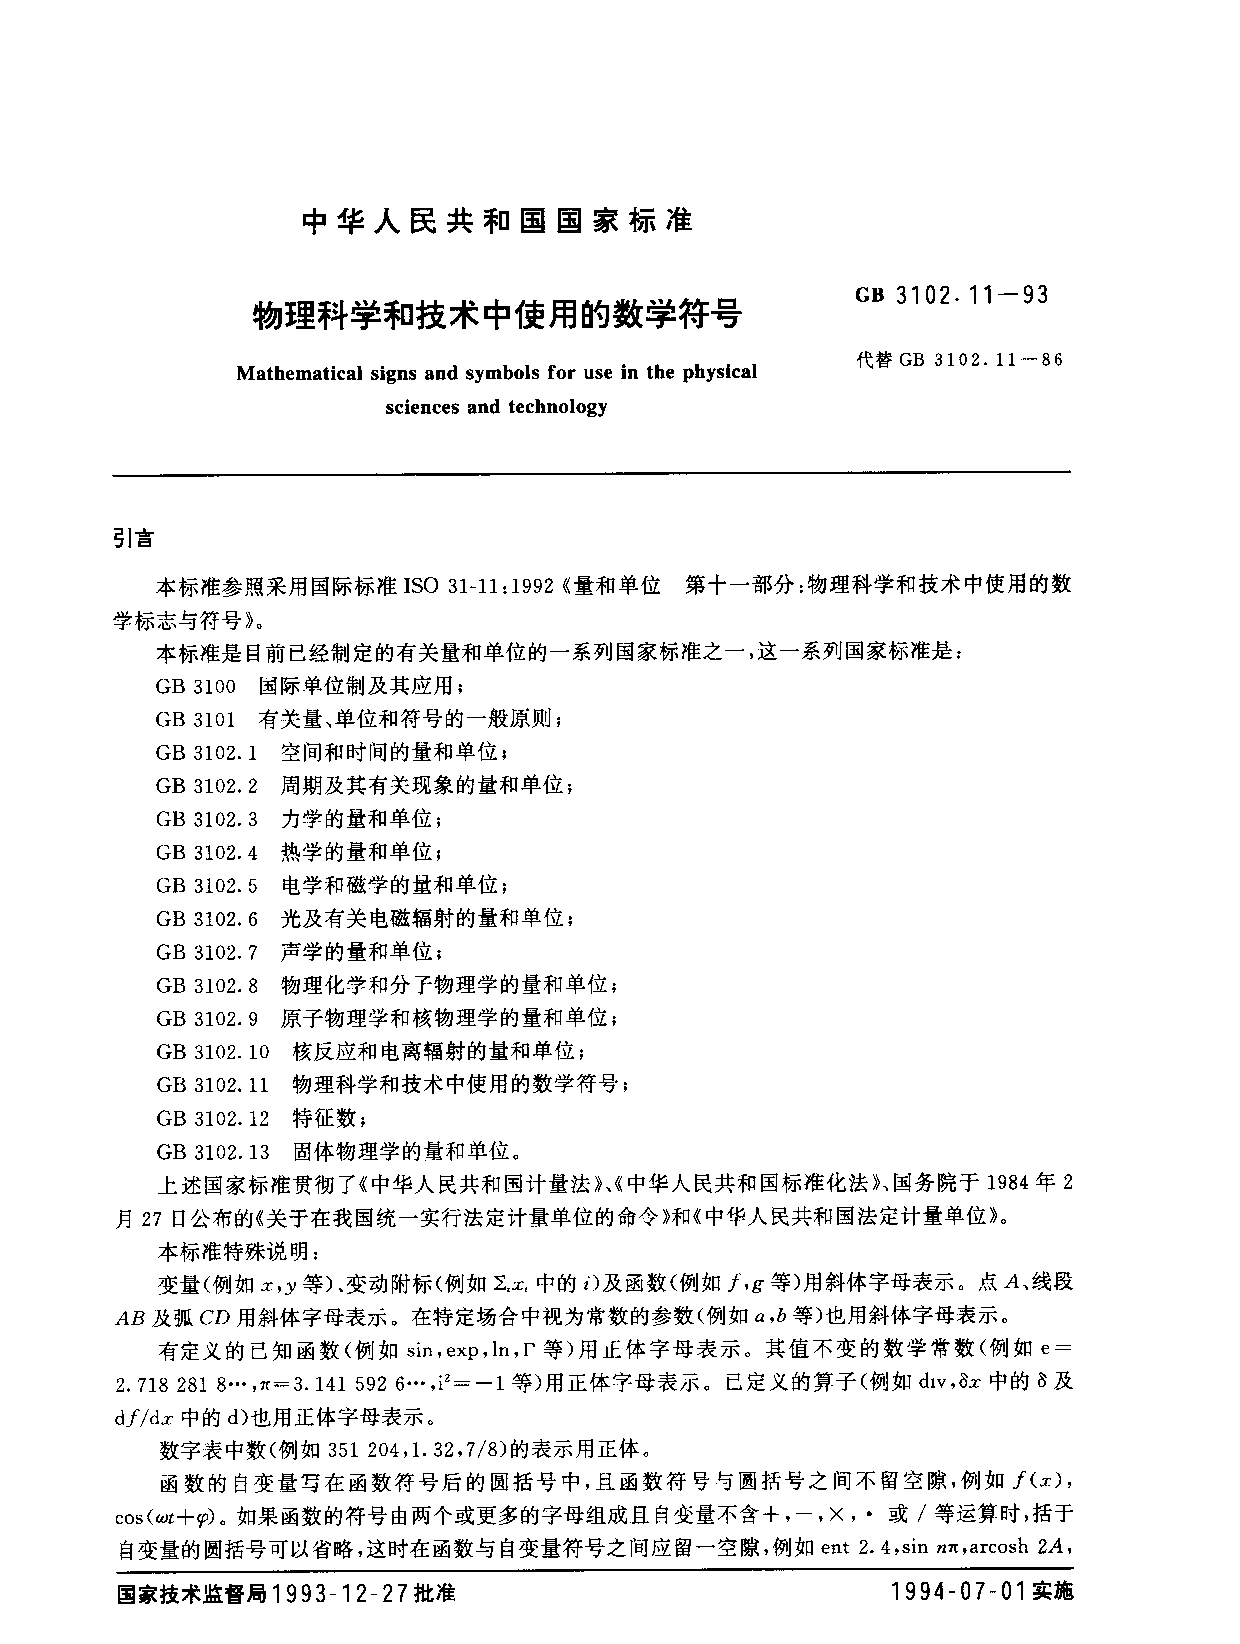
\includepdf[pages=-]{appendix/1993.pdf}
%!Mode::"TeX:UTF-8"

\defaultfont
\BiAppendixChapter{攻读学位期间取得的研究成果}{Achievements}

研究成果包括以下内容:
\begin{enumerate}
	\item 已发表或已录用的学术论文、已出版的专著/译著、已获授权的专利按参考文献格式列出。
	\item 科研获奖,列出格式为:获奖人(排名情况).项目名称.奖项名称及等级,发奖机构,获奖时间.
	\item 与学位论文相关的其它成果参照参考文献格式列出。
	\item 全部研究成果连续编号编排。
\end{enumerate}

\vspace{\baselineskip}
{\color{red}用于盲审的论文,只列出已发表学术论文的题目和刊物名称,可以备注自己为第几作者,及期刊影响因子。}

\clearpage{\pagestyle{empty}\cleardoublepage}%声明从奇数页开始

% !Mode:: "TeX:UTF-8"

\fancyhead[CO,CE]{\wuhao 声明}
\fancyfoot[LE,RO]{}
%\addcontentsline{toc}{chapter}{声\quad 明}
%\addcontentsline{toe}{chapter}{Statement of Copyright and Letter of Authorization}

\begin{center}\xiaowu\end{center}\vspace{-7mm}
\begin{center}\sanhao{学位论文独创性声明(1)}\end{center}

本人声明:所呈交的学位论文系在导师指导下本人独立完成的研究成果。文中依法引用他人的成果,均已做出明确标注或得到许可。论文内容未包含法律意义上已属于他人的任何形式的研究成果,也不包含本人已用于其他学位申请的论文或成果。

本人如违反上述声明,愿意承担以下责任和后果:
\begin{enumerate}
	\item 交回学校授予的学位证书;
	\item 学校可在相关媒体上对作者本人的行为进行通报;
	\item 本人按照学校规定的方式,对因不当取得学位给学校造成的名誉损害,进行公开道歉;
	\item 本人负责因论文成果不实产生的法律纠纷。
\end{enumerate}

\vspace{1em}
论文作者 (签名):\hfill 日期:\hspace{4em}年\hspace{3em}月\hspace{3em}日\hspace{4em}


\vspace{1em}
\begin{center}\sanhao{学位论文独创性声明(2)}\end{center}

本人声明:研究生\underline{\quad\quad\quad}所提交的本篇学位论文已经本人审阅,确系在本人指导下由该生独立完成的研究成果。

本人如违反上述声明,愿意承担以下责任和后果:
\begin{enumerate}
	\item 学校可在相关媒体上对本人的失察行为进行通报;
	\item 本人按照学校规定的方式,对因失察给学校造成的名誉损害,进行公开道歉;
	\item 本人接受学校按照有关规定做出的任何处理。
\end{enumerate}

\vspace{1em}
指导教师 (签名):\hfill 日期:\hspace{4em}年\hspace{3em}月\hspace{3em}日\hspace{4em}


\vspace{1em}
\begin{center}\sanhao{学位论文知识产权权属声明}\end{center}

我们声明,我们提交的学位论文及相关的职务作品,知识产权归属学校。学校享有以任何方式发表、复制、公开阅览、借阅以及申请专利等权利。学位论文作者离校后,或学位论文导师因故离校后,发表或使用学位论文或与该论文直接相关的学术论文或成果时,署名单位仍然为西安交通大学。

\vspace{1em}
论文作者 (签名):\hfill 日期:\hspace{4em}年\hspace{3em}月\hspace{3em}日\hspace{4em}

指导教师 (签名):\hfill 日期:\hspace{4em}年\hspace{3em}月\hspace{3em}日\hspace{4em}


\vspace{2em}
\noindent (本声明的版权归西安交通大学所有,未经许可,任何单位及任何个人不得擅自使用)


\end{document}
